\documentclass[aspectratio=169]{beamer}
\mode<presentation>
%\usetheme{Warsaw}
%\usetheme{Goettingen}
\usetheme{Hannover}
%\useoutertheme{default}

%\useoutertheme{infolines}
\useoutertheme{sidebar}
\usecolortheme{dolphin}


\setbeamersize{sidebar width left=0pt} % to remove the sidebar
\beamertemplatenavigationsymbolsempty % To remove the navigation symbols on the bottom right.
\setbeamersize{text margin left=10mm,text margin right=10mm} % Specify margins

\usepackage{amsmath}
\usepackage{amssymb}
\usepackage{listings}
\usepackage{enumerate}
\usepackage{hyperref}
\hypersetup{
    colorlinks=true,
    linkcolor=blue,
    filecolor=magenta,      
    urlcolor=cyan,
}
\usepackage{tikz}  %For grpah drawing 
 
\urlstyle{same}

%some bold math symbosl
\newcommand{\Cov}{\mathrm{Cov}}
\newcommand{\Var}{\mathrm{Var}}
\newcommand{\brho}{\boldsymbol{\rho}}
\newcommand{\bSigma}{\boldsymbol{\Sigma}}
\newcommand{\btheta}{\boldsymbol{\theta}}
\newcommand{\bbeta}{\boldsymbol{\beta}}
\newcommand{\bmu}{\boldsymbol{\mu}}
\newcommand{\bW}{\mathbf{W}}
\newcommand{\one}{\mathbf{1}}
\newcommand{\bH}{\mathbf{H}}
\newcommand{\by}{\mathbf{y}}
\newcommand{\bolde}{\mathbf{e}}
\newcommand{\bx}{\mathbf{x}}

\newcommand{\cpp}[1]{\texttt{#1}}

%--------------------------------------------------
\providecommand{\abs}[1]{\lvert#1\rvert}
\providecommand{\norm}[1]{\lVert#1\rVert}
\providecommand{\Blue}[1]{\textcolor{blue}{#1}}
\providecommand{\Red}[1]{\textcolor{red}{#1}}  
\providecommand{\Purple}[1]{\textcolor{purple}{#1}} %for notations
\newcommand{\celsius}{\ensuremath{^\circ}C}
\newcommand\thfore{\mathord{\therefore}\,}
%------------------------------------------------------------------

\title{Lecture 2. Fundamental Concepts and Terminologies}
\author{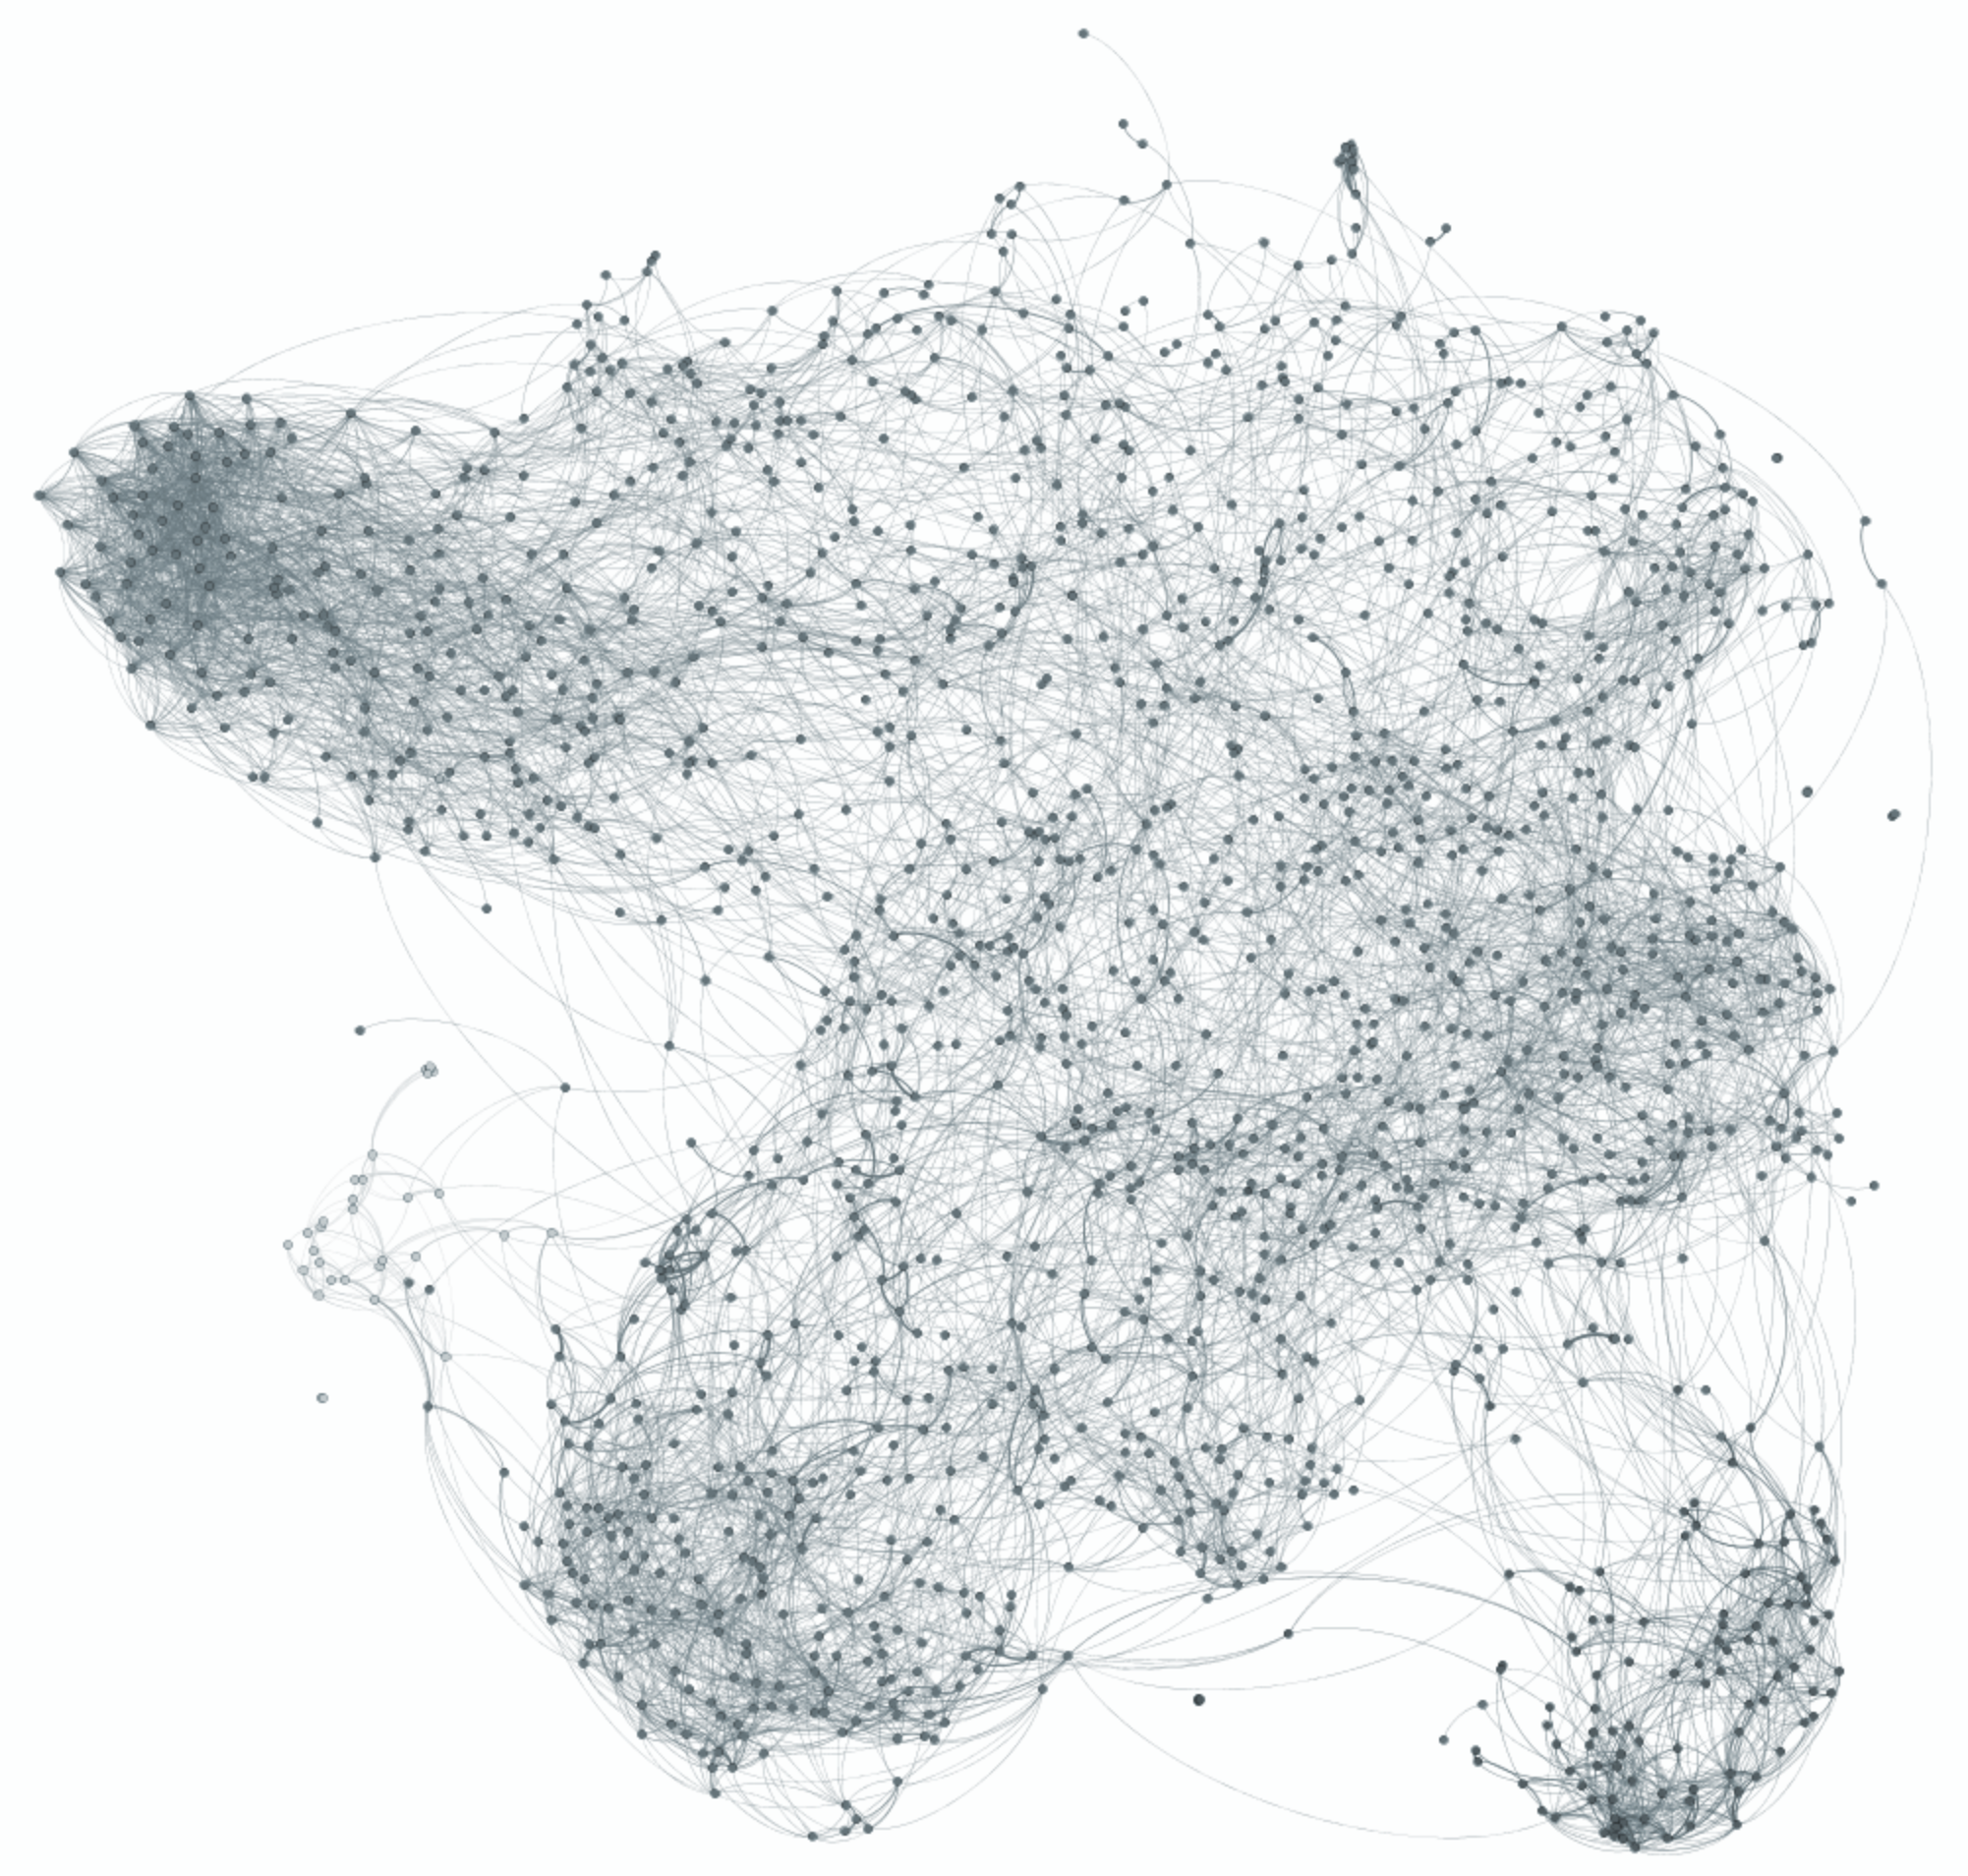
\includegraphics[width=.5\textwidth,height=.7\textheight]{./img/lecture2-fig0.png} \\
   \href{https://colah.github.io/posts/2014-07-FFN-Graphs-Vis/}{Graph of Harry Potter Fanfiction}
 }
 
\date{  }

\vspace{.3in}
%------------------------------------------------------------------


\begin{document}

\frame[plain]{\titlepage}


\begin{frame}[plain]{}
 
 {\bf Definition 2.1} A graph \Blue{$G = (V, E)$} consists of a nonempty set $V$ of {\bf vertices}
    (or {\bf nodes}) and a set $E$ of {\bf edges}.
    \begin{center}
      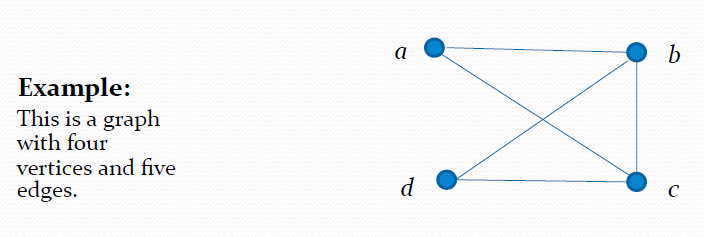
\includegraphics[height=3.5cm]{./img/lecture2-fig1.png}
    \end{center}
where $V = \{ a, b, c, d\}$ and $E = \{ (a,b), (a,c), (b,d), (b,c), (d,c)\} $. \\
\medskip

{\bf Remark}: Since the graph is undirected, $(a,b) = (b,a)$, $(a,c)=(c,a)$, etc.

\end{frame}

\begin{frame}[plain]{}

\Blue{Neighbors}: vertices $u$ and $v$ are \Blue{neighbors} (or called \Blue{adjacent})
 if an edge $(u,v)$ connects them.
\medskip

{\bf Example 2.2.}  $b$ and $c$ are neighbors.
 \begin{center}
      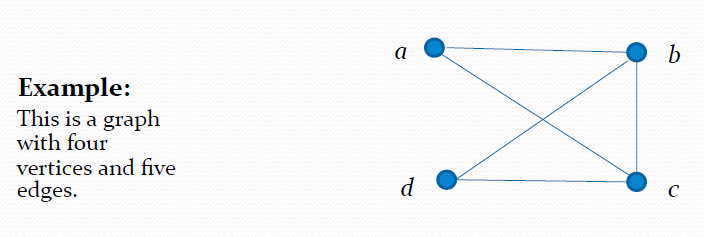
\includegraphics[height=3.5cm]{./img/lecture2-fig1.png}
    \end{center}
    
 {\bf Example 1.3.}  All neighbors of the node $a = \{ b, c\}$.
\end{frame}

\begin{frame}[plain]{}
 
   An edge that connects a vertex to itself is called a \Blue{loop}.
      \begin{center}
      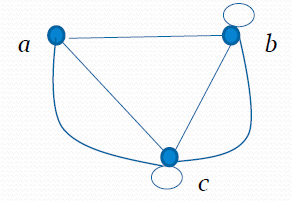
\includegraphics[height=3cm]{./img/lecture2-fig2.png}
    \end{center}
    
   The \Blue{degree} of a vertex is the number of edges connected to the vertex~\footnote{Equivalently, the number of neighbors of the vertex.}, 
   denoted by \Purple{deg(u)}.
   For example,
     in the figure above
     \begin{itemize}
       \item $\deg (a) =$ 
       \item $\deg (b) =$
       \item $\deg (c) = $
     \end{itemize}  \pause
     
   \Red{Notice} that a loop at a
vertex contributes two to the degree of that vertex.
 
\end{frame}

\begin{frame}[plain]{}
 
  {\bf Definition 2.4} An \Blue{directed graph}  
      \Blue{$G = (V, E)$} consists of a nonempty set $V$ of vertices 
      and a set $E$ of directed edges. %Each edge is
      %associated with an \Red{ordered pair of vertices}. The
      %directed edge associated with the ordered pair $(u,v)$ is
      %said to {\bf start at $u$} and {\bf end at $v$}. 
        \begin{center}
      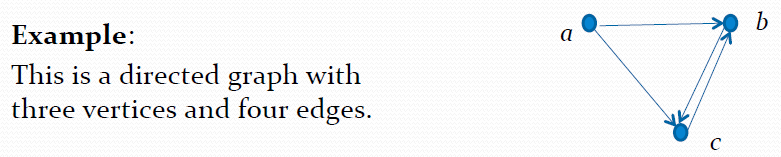
\includegraphics[height=2cm]{./img/lecture2-fig3.png}
    \end{center}
  %    \pause
     
 In a directed graph, 
      \begin{itemize}
        \item \Blue{Indegree} = the number of edges coming in to the vertex $v$ 
         (\Purple{$\deg^-(v)$})
        \item \Blue{Outdegree} = the number of edges going out of the vertex $v$ 
         (\Purple{$\deg^+(v)$})
      \end{itemize}
      
      \medskip
      
     \medskip

{\bf Remark}: $(a,b) \neq (b,a)$, $(b,c) \neq (c,b)$, etc.

\end{frame}

\begin{frame}[plain]{}
 
    {\bf Example 2.5.} Find the in-degree and out-degree of each vertex in the graph $G$ with
       directed edges shown in
       \medskip
       
       \begin{center}
         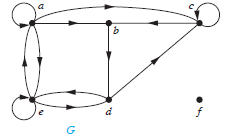
\includegraphics[height=3cm]{./img/lecture2-fig4.png}
       \end{center}
   \vspace{1in}
   
\end{frame}


\begin{frame}[plain]{}
 
   A \Blue{path} in a graph  $G$ is 
   a sequence of vertices $v_i$ and edges $e_i$ such that the edge $e_i$ connects vertices
   $v_{i-1}$ and $v_i$:
   \[ (v_0, e_1, v_1, e_2, v_2, ...,v_{n-1}, e_n, v_n) \]
   Equivalently,  assuming that two consecutive vertices are connected by an edge, we may write it without
   $e_i$'s
   \[ (v_0, v_1, v_2, ...,v_{n-1}, v_n) \]
   \pause
   \begin{itemize}
     \item The \Blue{length of a path} is the number of edges in the path.
      \item A \Blue{circuit} (or \Blue{cycle}) is  a path  
       that starts and ends on the same vertex ($v_0 = v_n$).
      \item A path or circuit is \Blue{simple} if it does not contain the same edge more than once.  \end{itemize}
  
\end{frame}

\begin{frame}[plain]{}
 
    {\bf Example 2.6.} In the graph
      \begin{center}
        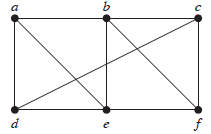
\includegraphics[height=3cm]{./img/lecture2-fig5.png}
      \end{center}
      \pause 
      \begin{itemize}[<+->]
       \item \Blue{$a, d, c, f, e$} is a simple path of length 4.
       \item  \Blue{$d, e, c, a$} is not a path because $e$ is not connected to $c$.
       \item \Blue{$b, c, f, e, b$} is a circuit of length 4.
       \item \Blue{$a, b, e, d, a, b$} is a path of length 5, but not a simple path.
       \end{itemize}
 
\end{frame}

\begin{frame}[plain]{}
 
 {\bf Example 2.7} 
    \begin{center}
        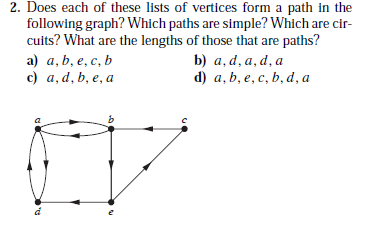
\includegraphics[height=5.5cm]{./img/lecture2-fig6.png}
      \end{center}  
\end{frame}

\begin{frame}[plain]{}
  \begin{itemize}
  \item An {\bf undirected} graph is \Blue{connected} if there is a path connecting any two vertices.
  \item A {\bf directed} graph is \Blue{connected} if the underlying undirected graph is. \pause 
  \item {\bf Example 2.8.} $G_1$ is connected because there is a path between
      any pair of its vertices, as can be easily seen. However $G_2$
      is not connected because there is no path between vertices
      $a$ and $f$, for example.
      \begin{center}
        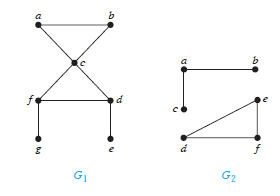
\includegraphics[height=4cm]{./img/lecture2-fig7.png}
      \end{center}
   \item \Blue{Connected component}: A subset of vertices $V_i\subset V$ that is connected. For example, in the above graph,
    $V_1 = \{ a,b,c\}$ and $V_2=\{ d,e,f\}$ are two connected components of $G_2$.
  \end{itemize}
\end{frame}

\begin{frame}[plain]{}

 {\bf Problem 2.9.} Is the graph below connected or not?
    \begin{center}
        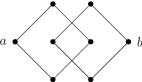
\includegraphics[height=2.5cm]{./img/lecture2-fig8.png}
      \end{center}
      
\end{frame}


    
\end{document}
%%%%%%%%%%%%%%%%%%%%%
 

